\documentclass[conference]{IEEEtran}
\IEEEoverridecommandlockouts
\usepackage{cite}
\usepackage{amsmath,amssymb,amsfonts}
\usepackage{graphicx}
\usepackage{booktabs}
\usepackage{multirow}
\usepackage{textcomp}
\usepackage{xcolor}
\usepackage{tikz}
\usetikzlibrary{arrows.meta,positioning}
\usepackage[hidelinks]{hyperref}
\graphicspath{{figures/}}

\begin{document}

\title{Predicting Cross-Source Matches of Noisy Business Records: Logistic, Discriminant and Count Models for Entity Resolution}

\author{
\IEEEauthorblockN{Manthan Vats}
\IEEEauthorblockA{Reg. No. 2427030314\\
Department of Computer Science and Engineering\\
UNIVERSITY NAME, CITY, India\\
EMAIL}
\and
\IEEEauthorblockN{Peddi Reddy Srikar Reddy}
\IEEEauthorblockA{Reg. No. 2427030741\\
Department of Computer Science and Engineering\\
UNIVERSITY NAME, CITY, India\\
EMAIL}
}

\maketitle

\begin{abstract}
Records of the same business often sit in several databases under different spellings, abbreviations and scripts,
with no shared identifier. We treat this entity resolution task as a predictive modeling problem on the Amazon ML
Challenge 2026 data, which links US and Indian business records across three sources. TF-IDF blocking reduces each
query to about 50 candidates, and every candidate pair is described by 43 engineered features. On a 5\% stratified
sample we compare logistic regression, linear and quadratic discriminant analysis and gradient boosting (LightGBM),
tuned by grid and random search under five-fold grouped cross-validation and tested on a lockbox of 21,685 entities.
LightGBM reaches a macro F0.5 of 0.9855 and logistic regression 0.9716, while LDA and QDA trail at 0.948 and 0.958.
The logistic coefficients show that address and house-number agreement, together with competition between entities
for the same record, predict a match better than name similarity. An expected-F0.5 decision rule beats fixed
probability thresholds for calibrated models. We also model the number of matches per entity: the counts are
under-dispersed (Pearson dispersion 0.31), so the negative binomial model collapses to the Poisson model, and a
multinomial logit classifies the counts more accurately. The full version of the pipeline scored 0.959 on the challenge
public leaderboard.
\end{abstract}

\begin{IEEEkeywords}
entity resolution, record linkage, logistic regression, discriminant analysis, gradient boosting, count regression, F-measure
\end{IEEEkeywords}

\section{Introduction}
Marketplaces, banks and logistics firms keep records of the same businesses in several systems, and those
systems rarely share an identifier. One source lists ``Sharma Traders Pvt Ltd, Plot 14, MG Road, Pune'', a second
writes ``Sharma Traders Private Limited, 14 Mahatma Gandhi Rd'' and a third gives the name in Devanagari with
no PIN code. Deciding which records belong to the same real business is called entity resolution (ER) or
record linkage~\cite{fellegi1969,christen2012}. Mistakes are expensive in both directions: a missed link splits
one seller into two accounts, while a false link merges the payment history of two unrelated companies.

We study ER as a predictive modeling problem. For each record of a reference source (Source~1) we must predict the
set of records in two other sources that describe the same business. The data is the training set of the Amazon
ML Challenge 2026 business entity resolution task: 2.2 million Source~1 records from the US and India,
10.3 million Source~2/3 records and 7.6 million labelled matches. Our team took part in the challenge with a
two-stage gradient boosting system that reached a public leaderboard score of 0.959 (macro F0.5).
For this paper we return to the problem with the tools of a predictive analytics course and ask three questions.
How far do interpretable classifiers (logistic regression, linear and quadratic discriminant analysis) get
compared with gradient boosting on the same features? Which evidence drives a match, as measured by the estimated
logistic regression coefficients? And can a count model for the number of matches per entity (Poisson, negative
binomial, multinomial logit) support the decision of how many candidates to accept?

The contributions are: (i) a reproducible pipeline that turns the raw records into 43 pair features after
TF-IDF blocking; (ii) a comparison of four classifiers with grouped cross-validation, grid search and random
search, scored on a lockbox split that was never touched while building the challenge system; (iii) an
analysis of decision rules that convert pair probabilities into match sets, including an expected-F0.5 rule;
and (iv) a count-data view of the problem, which shows that match counts in this data are under-dispersed.
All code, the executed notebook, the result tables and a dashboard are in our GitHub repository\footnote{\url{https://github.com/Manthan-Vats/carcosa-entity-resolution}. The challenge data belongs to the organisers; the repository holds only a 1,500-entity demo sample for the dashboard.}.

\section{Related Work}
The probabilistic basis of record linkage goes back to Fellegi and Sunter~\cite{fellegi1969}, who scored record pairs
by likelihood ratios of field agreement and accepted pairs above a threshold. Surveys by Elmagarmid
et al.~\cite{elmagarmid2007} and Christen~\cite{christen2012} describe the now standard steps: normalisation,
blocking, pair comparison, classification and evaluation. Blocking limits the quadratic number of comparisons;
Papadakis et al.~\cite{papadakis2020} review the main families, of which token and q-gram based similarity search
is closest to our TF-IDF approach~\cite{salton1988}.

Pair comparison relies on string similarity. Cohen et al.~\cite{cohen2003} compared edit-based and token-based
metrics for names and found hybrid token measures strongest, while the Jaro-Winkler metric~\cite{winkler1990}
remains common for short names. Bilenko and Mooney~\cite{bilenko2003} showed that learning how to combine
similarities with a classifier beats hand-tuned rules. Magellan~\cite{konda2016} packaged this
features-plus-classifier recipe, where random forests and logistic regression are typical choices. Deep models
followed: DeepMatcher~\cite{mudgal2018} and Ditto~\cite{li2020ditto} embed both records with neural or
pre-trained language models and gain most on textual, dirty data. They need GPUs and their decisions are harder to
explain, so we keep to feature-based models, where gradient boosted trees~\cite{friedman2001,ke2017} are the strongest
standard learner and logistic regression~\cite{hosmer2013} offers direct inference on each piece of evidence.

The challenge metric is an F-measure averaged over entities, so the decision step matters as much as the
probabilities. Lipton et al.~\cite{lipton2014} showed that the F1-optimal threshold of a calibrated classifier is
half the optimal F1 score, and Jansche~\cite{jansche2005} trained models directly for expected F-measure.
We use the expected-F idea per entity rather than one global threshold.

\section{Data and Preparation}
\subsection{Records and labels}
Each record has an identifier, a business name, an address and a country label. Source~1 is deduplicated; every
Source~2/3 record matches at most one Source~1 entity, and a Source~1 entity can match zero, one or many records.
The noise is typical of commercial data: legal suffix variants (Pvt/Private, Corp/Corporation), word order changes,
typos, DBA names, landmark addresses (``near SBI ATM''), missing PIN codes and, for India, names written in
Devanagari. Table~\ref{tab:quality} summarises missing addresses and non-Latin names in our sample.

\subsection{Normalisation}
Names and addresses are lower-cased, ``\&'' becomes ``and'', and text in Indic scripts is mapped to Latin with a token
dictionary learned from matched training pairs (1,339 name tokens), backed by a generic transliteration library
(\texttt{anyascii}) for unseen tokens. House and plot numbers are extracted into a separate field, and their
leading zeros are stripped (``00604'' $\rightarrow$ ``604''). Missing values are not imputed: an empty address
stays empty and is exposed to the models as a binary feature, and number features take the value $-1$ when either
record has no number, together with an explicit missing-number indicator. No outliers were removed. Unusually long
names (the 99th percentile is about 50 characters) are real records, and the length features capture them.

\subsection{Study sample and splits}
Running the full pipeline on all records takes several hours, so the comparative study uses a 5\% sample: 5\%
of the Source~1 entities, all their true matches, and 5\% of the Source~2/3 records that match nobody. Because
each Source~2/3 record belongs to at most one entity, the sample keeps the ratio of matched to unmatched records
(4.7 pool records per entity in both). The sample has 110,341 entities and 625,153 records in total.

The split unit is the Source~1 entity, so all candidate pairs of an entity fall in the same split. We reuse the
fold assignment of our challenge system: five development folds f0--f4 (16\% of entities each), stratified by
country and number of matches, and a 20\% lockbox. Folds f1--f3 train the final models, f4 serves for early
stopping and threshold choice, f0--f4 together form the five groups of the cross-validation used for tuning, and
the lockbox is the test set.

\begin{figure}[t]
\centering
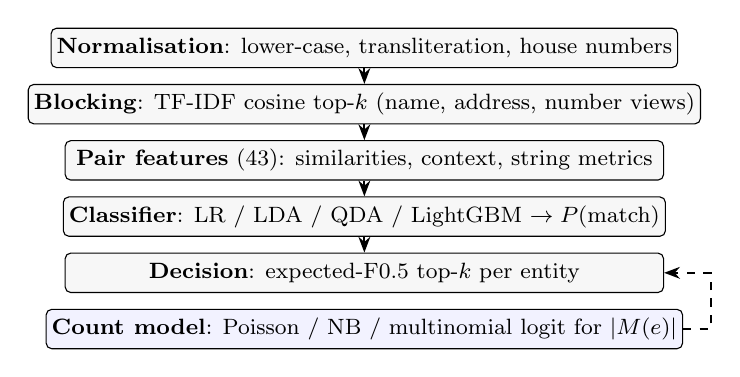
\begin{tikzpicture}[node distance=0.2cm, every node/.style={font=\footnotesize},
  box/.style={draw, rounded corners=2pt, align=center, minimum width=7.6cm, minimum height=0.5cm, inner sep=2pt, fill=gray!6},
  arr/.style={-{Stealth[length=2mm]}, thick}]
\node[box] (n) {\textbf{Normalisation}: lower-case, transliteration, house numbers};
\node[box, below=of n] (b) {\textbf{Blocking}: TF-IDF cosine top-$k$ (name, address, number views)};
\node[box, below=of b] (f) {\textbf{Pair features} (43): similarities, context, string metrics};
\node[box, below=of f] (c) {\textbf{Classifier}: LR / LDA / QDA / LightGBM $\rightarrow P(\text{match})$};
\node[box, below=of c] (d) {\textbf{Decision}: expected-F0.5 top-$k$ per entity};
\node[box, below=of d, fill=blue!5] (k) {\textbf{Count model}: Poisson / NB / multinomial logit for $|M(e)|$};
\draw[arr] (n) -- (b); \draw[arr] (b) -- (f); \draw[arr] (f) -- (c); \draw[arr] (c) -- (d);
\draw[arr, dashed] (k.east) -- ++(0.35,0) |- (d.east);
\end{tikzpicture}
\caption{Pipeline of the study. The count model is an alternative way to choose how many candidates to accept.}
\label{fig:pipeline}
\end{figure}

\section{Methodology}
\subsection{Blocking}
Comparing every Source~1 record with every pool record of the same country would mean about $10^{12}$ pairs on
the full data. Blocking keeps a short candidate list per entity. We build L2-normalised TF-IDF
vectors~\cite{salton1988} for four views: name character 3-grams (robust to typos), name words, address words and
house numbers. Very common terms are removed through a maximum document frequency (0.5\% for character
grams, 3\% for name words). For a weighted combination of views $v$ with weights $w_v$, the joint score of a
query $q$ and a pool record $r$ is
\begin{equation}
s(q,r)=\sum_{v} w_v \cos\!\big(\mathbf{x}^{(v)}_q,\mathbf{x}^{(v)}_r\big).
\end{equation}
Four searches with different weights (address-heavy, name-heavy, number-aware, and name-only among records without
an address) return their top 10--30 records, and the union forms the candidate set. Sparse top-$k$ matrix products
make this fast enough for a laptop CPU.

\subsection{Pair features}
Every candidate pair gets 43 features in four groups. \emph{Blocking similarities}: the four view cosines, the
joint score and the rank of the candidate in each search. \emph{Context}: the gap between a candidate's score and
the best score of the same entity, the gap to the best entity for the same candidate, ranks, and the number of
candidates per entity and per pool record. These features let a pointwise classifier see the competition among
candidates. \emph{String similarity}: Levenshtein ratio, token-sort and token-set ratios, partial ratio and
Jaro-Winkler on names~\cite{cohen2003,winkler1990}; token-set, token-sort and partial ratio on addresses; Jaccard
overlap and first-number agreement of house numbers. \emph{Record properties}: name and address lengths
(log-transformed), empty address, Devanagari script and candidate source.

For the linear and discriminant models we drop one feature of each pair with absolute Pearson correlation above 0.95
on the training folds, which removes redundant copies such as the joint score and its rank. Gradient boosting uses
all features.

\subsection{Classifiers}
\emph{Logistic regression} models the match probability of pair $i$ with feature vector $\mathbf{x}_i$ as
\begin{equation}
P(y_i=1\mid\mathbf{x}_i)=\sigma(\beta_0+\boldsymbol{\beta}^{\top}\mathbf{x}_i),\quad \sigma(z)=\frac{1}{1+e^{-z}},
\end{equation}
and the coefficients maximise the penalised log-likelihood
\begin{equation}
\ell(\boldsymbol\beta)=\sum_i\big[y_i\log p_i+(1-y_i)\log(1-p_i)\big]-\frac{1}{2C}\lVert\boldsymbol\beta\rVert_2^2 .
\end{equation}
For inference we refit an unpenalised model by maximum likelihood (Newton-Raphson) on standardised inputs, so that
$e^{\beta_j}$ is the odds ratio for a one standard deviation increase in feature $j$, and Wald $z$-tests give
standard errors and $p$-values~\cite{hosmer2013}.

\emph{Linear discriminant analysis} assumes Gaussian class densities with a shared covariance $\Sigma$ and classifies by
\begin{equation}
\delta_k(\mathbf{x})=\mathbf{x}^{\top}\Sigma^{-1}\boldsymbol\mu_k-\tfrac12\boldsymbol\mu_k^{\top}\Sigma^{-1}\boldsymbol\mu_k+\log\pi_k ,
\end{equation}
which gives a linear boundary~\cite{fisher1936,hastie2009}. We tune Ledoit-Wolf style shrinkage of
$\Sigma$~\cite{ledoit2004}. \emph{Quadratic discriminant analysis} allows a covariance $\Sigma_k$ per class, which
adds the term $-\tfrac12\log|\Sigma_k|$ and makes the boundary quadratic; its regularisation parameter shrinks
each $\Sigma_k$ towards the identity. \emph{LightGBM}~\cite{ke2017} fits an additive model of regression trees by
gradient boosting on the log-loss~\cite{friedman2001} and serves as the non-linear reference, since it is the model
of our challenge system.

\subsection{From probabilities to match sets}
The challenge score of entity $e$ with predicted set $\hat M$ and true set $M$ is
\begin{equation}
F_{0.5}(e)=\frac{(1+\beta^2)\,PR}{\beta^2P+R},\quad \beta=0.5,
\end{equation}
with precision $P=|\hat M\cap M|/|\hat M|$ and recall $R=|\hat M\cap M|/|M|$. An entity without matches scores 1
only when nothing is predicted, and the final score is the mean over entities. $\beta=0.5$ weighs precision twice
as much as recall. We compare three rules: a fixed threshold of 0.5; the threshold that maximises pair-level F1 on
f4; and an \emph{expected-F0.5 top-$k$} rule. With candidate probabilities sorted as $p_1\ge p_2\ge\dots$, the
rule picks
\begin{equation}
k^{*}=\arg\max_{k\ge 1}\frac{1.25\sum_{j\le k}p_j}{k+0.25\sum_j p_j},
\end{equation}
a ratio-of-expectations approximation of the expected F0.5, and predicts the empty set instead when
$\prod_j(1-p_j)$, the probability that the entity has no match among its candidates, is larger.

\subsection{Count models}
Let $N_e=|M(e)|$ be the number of true matches of entity $e$. From eight entity-level summaries of the candidate
list (counts of strong name and address agreements, the best joint and name scores, record lengths and country) we
fit a Poisson GLM with log link, $\log \mathbb{E}[N_e]=\mathbf{z}_e^{\top}\boldsymbol\gamma$, and a negative
binomial (NB2) model with $\operatorname{Var}(N_e)=\mu_e+\alpha\mu_e^2$, which relaxes the Poisson assumption
that the variance equals the mean~\cite{cameron2013}. A multinomial logit over the classes $\{0,1,2,3{+}\}$ treats
the count as a category. The predicted mean also gives a decision rule: accept the $\operatorname{round}(\hat\mu_e)$
highest-ranked candidates.

\subsection{Validation and tuning}
Hyperparameters are tuned by five-fold grouped cross-validation~\cite{kohavi1995} on 15,000 development entities
(about 790k pairs), with the predefined folds as groups so that no entity is split. Grid search covers the
logistic regression penalty $C\in\{10^{-3},\dots,10\}$ with and without class weighting, LDA shrinkage, and the QDA
regularisation parameter. For LightGBM, random search~\cite{bergstra2012} draws 12 settings of the number of leaves,
learning rate, minimum leaf size, row and column subsampling and L2 penalty. The tuning score is average precision,
because only about 6.5\% of the pairs are matches and accuracy or ROC-AUC alone would hide differences in
precision~\cite{saito2015}. Pair-level results are reported as AUC-ROC, PR-AUC, F1, precision, recall, log-loss and
Brier score; count models as MAE and RMSE. All models use scikit-learn~\cite{pedregosa2011},
statsmodels~\cite{seabold2010} and LightGBM.

\section{Experiments and Results}
\subsection{Setup}
Blocking on the study sample returned 5.80 million candidate pairs, 52.5 per entity, and kept 99.4\% of the true
matches. Positives make up 6.5\% of the pairs. The final models are trained on 2.78M pairs (52,967 entities in
f1--f3), validated on 0.93M pairs (f4) and tested on 1.14M pairs from 21,685 lockbox entities. The correlation filter
removed five of the 43 features for the linear and discriminant models (address token-sort and partial ratio, the
candidate address length, first-number agreement, and one gap feature). Everything ran on a 16-thread laptop CPU;
the tuning stage took 19 minutes and the largest single fit, LightGBM, about two minutes.

\begin{table}[t]
\centering
\footnotesize
\caption{Data quality of the study sample (name length: median characters)}
\label{tab:quality}
\begin{tabular}{llrrr}
\toprule
Src. & Country & Empty addr. \% & Devanagari \% & Name len. \\
\midrule
S1 & India & 0.0 & 0.0 & 27 \\
S1 & US & 0.0 & 0.0 & 22 \\
S2 & India & 2.9 & 23.5 & 27 \\
S2 & US & 3.6 & 0.0 & 23 \\
S3 & India & 3.0 & 13.2 & 27 \\
S3 & US & 3.5 & 0.0 & 23 \\
\bottomrule
\end{tabular}
\end{table}


\subsection{Exploratory analysis}
The two countries look alike in structure. About 3--4\% of Source~2/3 records have no address, while Source~1
addresses are always present (Table~\ref{tab:quality}). Devanagari appears only in Indian records: 23.5\% of
Source~2 names and 13.2\% of Source~3 names. Fig.~\ref{fig:counts} shows the number of true matches per entity.
The mode is three, 5.6\% of entities have no match at all, and the distributions of the two countries almost
coincide. The mean is 3.45 and the variance 2.88, a first sign that a Poisson model, whose variance equals its
mean, will not fit well. Fig.~\ref{fig:dist} contrasts three similarity features. Matches pile up near the
maximum, but a fair share of non-matches also have identical names (the right-hand spike of the name cosine),
because chain stores and common trade names repeat across cities. The address
similarity separates the classes better, which the coefficients below confirm.

\begin{figure}[t]
\centering
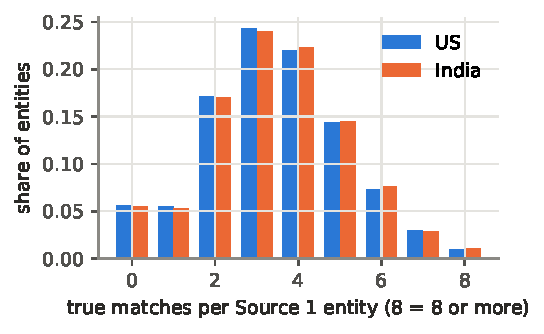
\includegraphics[width=0.75\linewidth]{fig_match_counts}
\caption{Distribution of the number of true matches per Source~1 entity.}
\label{fig:counts}
\end{figure}

\begin{figure*}[t]
\centering
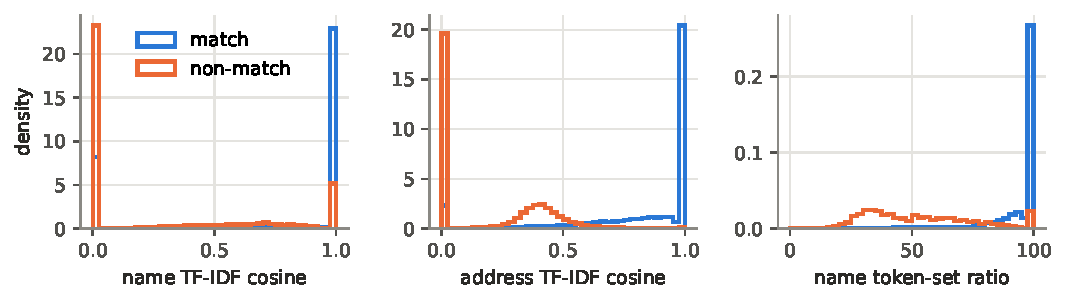
\includegraphics[width=0.72\textwidth]{fig_feature_dist}
\caption{Densities of three pair features for matching and non-matching candidates (400k random pairs).}
\label{fig:dist}
\end{figure*}

\subsection{Tuning}
Table~\ref{tab:tuning} lists the selected settings. Logistic regression is flat across $C\ge0.1$
(average precision 0.9973--0.9974) and class weighting did not help, so the default $C=1$ without weights was
kept. LDA worked best without shrinkage, which is expected with 790k rows and 38 features. QDA needed
regularisation ($0.1$): without it the per-class covariance of the matches is close to singular. The random
search for LightGBM chose 85 leaves and a learning rate of 0.052, and early stopping on f4 ended the final fit
after 541 trees. Cross-validation standard deviations are at most 0.001, so the ranking of the models is
stable across folds.

\begin{table}[t]
\centering
\footnotesize
\caption{Hyperparameter search with 5-fold grouped cross-validation}
\label{tab:tuning}
\begin{tabular}{llll}
\toprule
Model & Search & Selected setting & CV AP (mean $\pm$ sd) \\
\midrule
LR & grid & $C=1$, weights: none & 0.9974 $\pm$ 0.0001 \\
LDA & grid & shrinkage: none & 0.9857 $\pm$ 0.0009 \\
QDA & grid & reg. param $=0.1$ & 0.9917 $\pm$ 0.0004 \\
LightGBM & random & 85 leaves, lr 0.052 & 0.9991 $\pm$ 0.0001 \\
\bottomrule
\end{tabular}
\end{table}

\begin{table*}[t]
\centering
\footnotesize
\caption{Pair-level results on the lockbox (1.14M pairs, F1 threshold chosen on f4)}
\label{tab:pairs}
\begin{tabular}{lrrrrrrr}
\toprule
Model & AUC-ROC & PR-AUC & F1 & Prec. & Rec. & Log-loss & Brier \\
\midrule
LR & 0.9998 & 0.9972 & 0.9786 & 0.9733 & 0.9840 & 0.0081 & 0.0022 \\
LDA & 0.9983 & 0.9845 & 0.9460 & 0.9676 & 0.9253 & 0.0760 & 0.0066 \\
QDA & 0.9987 & 0.9884 & 0.9690 & 0.9677 & 0.9704 & 0.0386 & 0.0042 \\
LightGBM & \textbf{1.0000} & \textbf{0.9993} & \textbf{0.9885} & \textbf{0.9893} & \textbf{0.9878} & \textbf{0.0041} & \textbf{0.0011} \\
\bottomrule
\end{tabular}
\end{table*}


\subsection{Pair-level classification}
All four models separate the classes well by AUC-ROC (Table~\ref{tab:pairs}), with values between 0.998 and 1.000.
That number hides the differences that matter, because with 1.07 million negatives even a false positive rate of
0.2\% means two thousand wrong links. The precision-recall view and Fig.~\ref{fig:roc} are more telling. LightGBM
reaches an F1 of 0.989 and makes 797 false positives, against 2,011 for logistic regression, 2,303 for LDA and 2,412
for QDA. Logistic regression is the best of the classical models on every metric (F1 0.979), and its log-loss of
0.008 shows well calibrated probabilities. LDA has the lowest recall (0.925), since its single shared covariance
cannot fit the very different spread of the two classes. QDA ranks pairs well but its probabilities are extreme: its
F1-optimal threshold is 0.987 and its log-loss five times that of logistic regression.

\begin{figure*}[t]
\centering
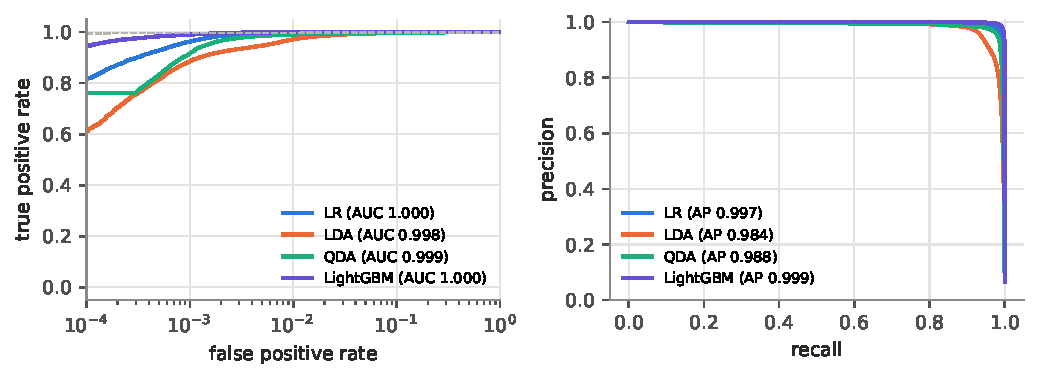
\includegraphics[width=0.66\textwidth]{fig_roc_pr}
\caption{ROC curves (log-scaled false positive rate) and precision-recall curves on the lockbox.}
\label{fig:roc}
\end{figure*}

\subsection{What drives a match}
The maximum likelihood fit on 250k training pairs reaches a McFadden pseudo-$R^2$ of 0.948. Fig.~\ref{fig:coef}
plots the standardised coefficients. Three findings stand out. First, the strongest predictor is a context
feature, \texttt{joint\_gap\_cand} ($\hat\beta=5.73$, $p<10^{-100}$): a record that resembles another Source~1
entity better than the current one is unlikely to belong to the current one. Since each Source~2/3 record has a
single owner, competition between entities carries more information than any single similarity. Second,
address agreement outweighs name agreement. The address token-set ratio has an odds ratio of 45 per standard
deviation and house-number overlap one of 25, while name TF-IDF cosine has 1.45 once the string metrics are present.
Address cosine is only borderline ($p=0.015$) and the gap to the entity's best candidate is not significant
($p=0.40$). Third, a Devanagari candidate is less likely to match at the same similarity level
(odds ratio 0.67), which suggests that transliteration makes non-matching names look more alike than they are.
The large positive coefficients of \texttt{num\_missing} and \texttt{c\_addr\_empty} should be read together with
the features they flag: they offset the $-1$ code and the zero similarity that a missing value produces, and are not
evidence that missing data indicates a match.

\begin{figure}[t]
\centering
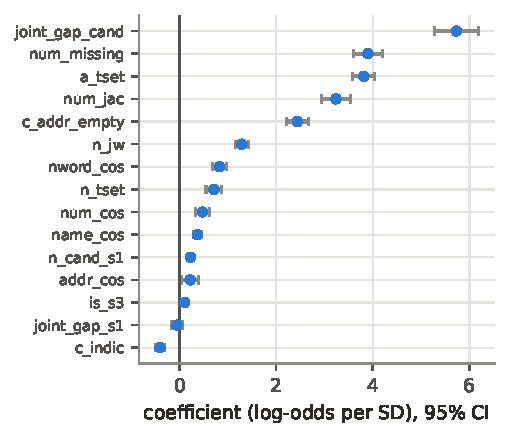
\includegraphics[width=0.8\linewidth]{fig_logit_coef}
\caption{Logistic regression coefficients on standardised features with 95\% Wald intervals.}
\label{fig:coef}
\end{figure}

\begin{table}[t]
\centering
\footnotesize
\caption{Entity-level macro F0.5 on the lockbox (21,685 entities); US/India use the expected-F0.5 rule}
\label{tab:entity}
\begin{tabular}{lrrrrr}
\toprule
Model & $p\ge0.5$ & F1 thr. & Exp.-F0.5 & US & India \\
\midrule
LR & 0.9703 & 0.9683 & 0.9716 & 0.9720 & 0.9710 \\
LDA & 0.9473 & 0.9475 & 0.9477 & 0.9564 & 0.9348 \\
QDA & 0.9476 & 0.9581 & 0.9512 & 0.9604 & 0.9374 \\
LightGBM & 0.9840 & 0.9843 & \textbf{0.9855} & 0.9869 & 0.9834 \\
\midrule
\multicolumn{6}{l}{Perfect classifier on the blocked candidates: 0.9979} \\
\bottomrule
\end{tabular}
\end{table}


\subsection{Entity-level results}
Table~\ref{tab:entity} reports the challenge metric. LightGBM with the expected-F0.5 rule scores 0.9855, within
0.013 of the 0.9979 ceiling set by blocking. Logistic regression reaches 0.9716, QDA 0.9581 and LDA 0.9477. The
decision rule matters in a model-dependent way. For the two calibrated models the expected-F0.5 rule is best:
it adapts the number of accepted candidates to each entity and predicts nothing when no candidate is convincing.
For logistic regression the F1 threshold (0.39) is even worse than 0.5, because it trades precision for recall
while F0.5 rewards the opposite. For QDA the expected-F0.5 rule loses to the threshold, as the rule takes
probabilities at face value and QDA's are badly calibrated. Indian entities score 0.1--2.3 points lower than US
ones for every model, which matches the extra script and spelling noise seen in Table~\ref{tab:quality}.

\subsection{Overfitting and underfitting}
Fig.~\ref{fig:overfit} shows both failure modes. On the left, a deliberately flexible LightGBM (255 leaves, five
samples per leaf) drives the training log-loss to $4\times10^{-8}$, while the validation log-loss reaches its minimum
of 0.0054 at round 87 and then nearly doubles to 0.0102 by round 800. Early stopping and the tuned leaf size of 97
avoid this. On the right, a single decision tree underfits at small depths (average precision 0.81 at depth one on both
sets), peaks on validation at depth eight (0.988), and overfits beyond it: at depth 24 and above the tree reproduces
the training data exactly while validation precision drops to 0.951.

\begin{figure*}[t]
\centering
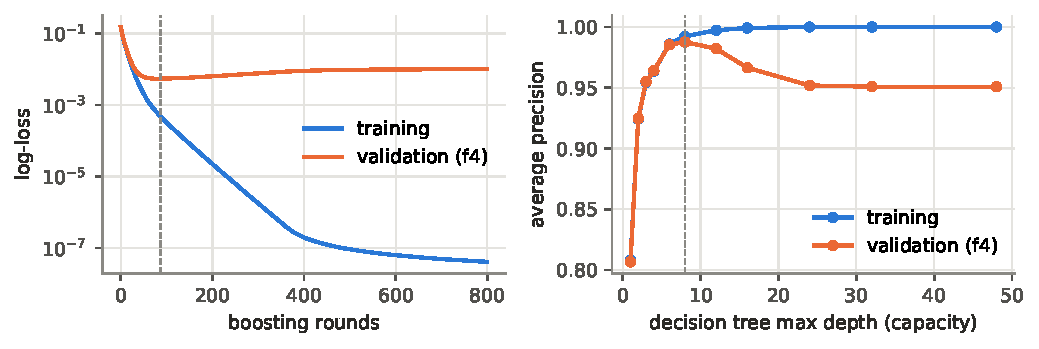
\includegraphics[width=0.66\textwidth]{fig_overfit}
\caption{Left: training and validation log-loss of an over-flexible LightGBM; the dashed line marks the validation
minimum. Right: average precision of a decision tree against its maximum depth.}
\label{fig:overfit}
\end{figure*}

\begin{table}[t]
\centering
\footnotesize
\caption{Count models for the number of matches per entity (lockbox). The multinomial logit predicts capped classes, so its MAE/RMSE are on the 0--3 scale}
\label{tab:counts}
\begin{tabular}{lrrrr}
\toprule
Model & AIC & MAE & RMSE & Acc. (0/1/2/3+) \\
\midrule
Poisson GLM & 288,006 & 0.713 & 0.949 & 0.763 \\
Negative binomial & 288,008 & 0.713 & 0.949 & 0.763 \\
Multinomial logit & 77,703 & 0.211 & 0.506 & 0.808 \\
\bottomrule
\end{tabular}
\end{table}


\subsection{Count models}
The Poisson GLM finds sensible effects: the count rises with the number of candidates that agree strongly on both
name and address ($\hat\gamma=0.60$ on the log scale) and with the best name similarity, and is about 10\% lower for
Indian entities at equal evidence. Its fit, however, shows strong under-dispersion: the Pearson statistic divided
by the residual degrees of freedom is 0.31, far below the value of one implied by the model. The negative binomial
can only add variance, so its dispersion parameter collapses to $\hat\alpha\approx2\times10^{-8}$ and it reproduces
the Poisson fit almost exactly (Table~\ref{tab:counts}). The source of under-dispersion is plain: most entities have
two to five matches and few have none or many, so the counts are more regular than independent events would be.
Treating the count as a category works better. The multinomial logit over $\{0,1,2,3{+}\}$ classifies 80.8\% of
the lockbox entities correctly, against 76.3\% for the rounded Poisson mean on the same classes.

Used as a decision rule, the count model falls well short. Accepting the top $\operatorname{round}(\hat\mu)$
LightGBM candidates gives a macro F0.5 of only 0.860, against 0.9855 for the expected-F0.5 rule. A mean absolute
count error of 0.71 is small for a regression, but every unit of error is a missed or wrong link. The pair
probabilities already contain sharper information about each entity than eight summary statistics do.

\begin{table*}[t]
\centering
\footnotesize
\caption{Development of the full challenge system (all 1.76M dev entities, scored on fold f0)}
\label{tab:challenge}
\begin{tabular}{llrrrr}
\toprule
Run & Change & Dev F0.5 & Recall cap & Cands/S1 & Public LB \\
\midrule
r001 & TF-IDF top-15, LightGBM prune + pair model & 0.9364 & 0.8881 & 4.27 & 0.902 \\
r002 & union blocking, transliteration, sibling features & 0.9546 & 0.9346 & 5.59 & 0.927 \\
r003 & r002 with stage B on more data & 0.9535 & 0.9346 & 5.59 & -- \\
r004 & name-word view, cross-fitted stage A & 0.9742 & 0.9732 & 5.14 & 0.959 \\
\bottomrule
\end{tabular}
\end{table*}


\subsection{The full challenge system}
Table~\ref{tab:challenge} traces our challenge entry on the full data, where each entity competes with 20 times
more look-alikes. The largest gains came from blocking, not from the classifier: union blocking and transliteration
raised the recall ceiling from 0.888 to 0.935, and a name-word TF-IDF view raised it to 0.973, lifting the dev score
from 0.936 to 0.974 and the public leaderboard score from 0.902 to 0.959. Training the second stage on more data
(r003) did not help. The two-stage design keeps the candidate file small (5.1 candidates per entity), which the
challenge rewarded separately.

\section{Discussion}
The comparison gives a clear order: gradient boosting first, then logistic regression, QDA and LDA. Logistic
regression is the practical runner-up. It is 1.4 points behind LightGBM on the challenge metric, trains in eleven
seconds instead of two minutes, and every coefficient can be read and tested. In a setting where links must be
explained to a reviewer or an auditor, that trade may be worth making. The discriminant models suffer from the
Gaussian assumption. Similarity scores are bounded and pile up at their maximum (Fig.~\ref{fig:dist}), which is
far from normal, so LDA and QDA lose recall and calibration respectively.

Two lessons carry beyond this data. First, a metric that averages over entities must be optimised over entities:
a fixed pair threshold, even one tuned for F1, leaves score on the table, while the expected-F0.5 rule needs only
calibrated probabilities. Second, checking the dispersion of a count before choosing between Poisson and negative
binomial is not a formality. Here the usual remedy for a poor Poisson fit, the negative binomial, cannot help,
because the problem is too little variance rather than too much.

\subsection{Ethical considerations}
Business records are less sensitive than personal data, but ER systems in practice also link sole proprietors,
whose business name is often a person's name and whose address is a home. A false merge can attach one trader's
complaints or credit history to another, and the harm falls on the smaller party, who may not know the link
exists. For that reason we favour a precision-weighted metric, keep the model's evidence inspectable through the
logistic regression coefficients and the dashboard, and recommend human review for low-confidence links before they
change any account. The model performs slightly worse on Indian records, which carry more script and spelling
variation; a deployed system should monitor error rates per country and script so that one group of businesses
does not bear most of the mistakes. The challenge data is used only for this academic study; apart from a small demo
sample for the dashboard, it is not redistributed.

\subsection{Limitations}
The study sample keeps the ratio of matched to unmatched records but has 20 times fewer records per country, so
each entity faces fewer look-alike competitors. Blocking recall is therefore higher (99.4\%) than on the full data
(97.8\%), and absolute scores are optimistic compared with the full challenge setting. The comparison between
models is still fair, because all of them see the same candidates and features. The test countries of the
challenge include France, which is absent from training; the lockbox only contains US and Indian records, so our
results say nothing direct about transfer to a new country. Time series methods from the syllabus do not apply,
since the records carry no timestamps.


\section{Conclusion}
We treated business entity resolution as a predictive modeling problem: TF-IDF blocking, 43 engineered pair
features, four classifiers tuned with grouped cross-validation, an entity-level decision rule and count models for
the number of matches. On a held-out lockbox of 21,685 entities, LightGBM reached a macro F0.5 of 0.9855 and logistic
regression 0.9716, against a ceiling of 0.9979. The logistic coefficients show that address and house-number
agreement and the competition between entities for a record matter more than name similarity. The match counts are
under-dispersed, so the negative binomial model reduces to Poisson and a multinomial logit fits better, but no count
model beats the expected-F0.5 rule as a way to choose matches. The full version of the pipeline reached 0.959 on the
Amazon ML Challenge 2026 public leaderboard. Future work includes testing transfer to unseen countries such as
France, ordinal or generalised Poisson models for under-dispersed counts, and calibrating QDA before using it in the
expected-F rule.


\bibliographystyle{IEEEtran}
\bibliography{refs}


\end{document}
